% Options for packages loaded elsewhere
\PassOptionsToPackage{unicode}{hyperref}
\PassOptionsToPackage{hyphens}{url}
%
\documentclass[
  english,
  man,floatsintext]{apa6}
\usepackage{lmodern}
\usepackage{amssymb,amsmath}
\usepackage{ifxetex,ifluatex}
\ifnum 0\ifxetex 1\fi\ifluatex 1\fi=0 % if pdftex
  \usepackage[T1]{fontenc}
  \usepackage[utf8]{inputenc}
  \usepackage{textcomp} % provide euro and other symbols
\else % if luatex or xetex
  \usepackage{unicode-math}
  \defaultfontfeatures{Scale=MatchLowercase}
  \defaultfontfeatures[\rmfamily]{Ligatures=TeX,Scale=1}
\fi
% Use upquote if available, for straight quotes in verbatim environments
\IfFileExists{upquote.sty}{\usepackage{upquote}}{}
\IfFileExists{microtype.sty}{% use microtype if available
  \usepackage[]{microtype}
  \UseMicrotypeSet[protrusion]{basicmath} % disable protrusion for tt fonts
}{}
\makeatletter
\@ifundefined{KOMAClassName}{% if non-KOMA class
  \IfFileExists{parskip.sty}{%
    \usepackage{parskip}
  }{% else
    \setlength{\parindent}{0pt}
    \setlength{\parskip}{6pt plus 2pt minus 1pt}}
}{% if KOMA class
  \KOMAoptions{parskip=half}}
\makeatother
\usepackage{xcolor}
\IfFileExists{xurl.sty}{\usepackage{xurl}}{} % add URL line breaks if available
\IfFileExists{bookmark.sty}{\usepackage{bookmark}}{\usepackage{hyperref}}
\hypersetup{
  pdftitle={The title},
  pdfauthor={First Author1 \& Ernst-August Doelle1,2},
  pdflang={en-EN},
  pdfkeywords={keywords},
  hidelinks,
  pdfcreator={LaTeX via pandoc}}
\urlstyle{same} % disable monospaced font for URLs
\usepackage{graphicx}
\makeatletter
\def\maxwidth{\ifdim\Gin@nat@width>\linewidth\linewidth\else\Gin@nat@width\fi}
\def\maxheight{\ifdim\Gin@nat@height>\textheight\textheight\else\Gin@nat@height\fi}
\makeatother
% Scale images if necessary, so that they will not overflow the page
% margins by default, and it is still possible to overwrite the defaults
% using explicit options in \includegraphics[width, height, ...]{}
\setkeys{Gin}{width=\maxwidth,height=\maxheight,keepaspectratio}
% Set default figure placement to htbp
\makeatletter
\def\fps@figure{htbp}
\makeatother
\setlength{\emergencystretch}{3em} % prevent overfull lines
\providecommand{\tightlist}{%
  \setlength{\itemsep}{0pt}\setlength{\parskip}{0pt}}
\setcounter{secnumdepth}{-\maxdimen} % remove section numbering
% Make \paragraph and \subparagraph free-standing
\ifx\paragraph\undefined\else
  \let\oldparagraph\paragraph
  \renewcommand{\paragraph}[1]{\oldparagraph{#1}\mbox{}}
\fi
\ifx\subparagraph\undefined\else
  \let\oldsubparagraph\subparagraph
  \renewcommand{\subparagraph}[1]{\oldsubparagraph{#1}\mbox{}}
\fi
% Manuscript styling
\usepackage{upgreek}
\captionsetup{font=singlespacing,justification=justified}

% Table formatting
\usepackage{longtable}
\usepackage{lscape}
% \usepackage[counterclockwise]{rotating}   % Landscape page setup for large tables
\usepackage{multirow}		% Table styling
\usepackage{tabularx}		% Control Column width
\usepackage[flushleft]{threeparttable}	% Allows for three part tables with a specified notes section
\usepackage{threeparttablex}            % Lets threeparttable work with longtable

% Create new environments so endfloat can handle them
% \newenvironment{ltable}
%   {\begin{landscape}\begin{center}\begin{threeparttable}}
%   {\end{threeparttable}\end{center}\end{landscape}}
\newenvironment{lltable}{\begin{landscape}\begin{center}\begin{ThreePartTable}}{\end{ThreePartTable}\end{center}\end{landscape}}

% Enables adjusting longtable caption width to table width
% Solution found at http://golatex.de/longtable-mit-caption-so-breit-wie-die-tabelle-t15767.html
\makeatletter
\newcommand\LastLTentrywidth{1em}
\newlength\longtablewidth
\setlength{\longtablewidth}{1in}
\newcommand{\getlongtablewidth}{\begingroup \ifcsname LT@\roman{LT@tables}\endcsname \global\longtablewidth=0pt \renewcommand{\LT@entry}[2]{\global\advance\longtablewidth by ##2\relax\gdef\LastLTentrywidth{##2}}\@nameuse{LT@\roman{LT@tables}} \fi \endgroup}

% \setlength{\parindent}{0.5in}
% \setlength{\parskip}{0pt plus 0pt minus 0pt}

% \usepackage{etoolbox}
\makeatletter
\patchcmd{\HyOrg@maketitle}
  {\section{\normalfont\normalsize\abstractname}}
  {\section*{\normalfont\normalsize\abstractname}}
  {}{\typeout{Failed to patch abstract.}}
\patchcmd{\HyOrg@maketitle}
  {\section{\protect\normalfont{\@title}}}
  {\section*{\protect\normalfont{\@title}}}
  {}{\typeout{Failed to patch title.}}
\makeatother
\shorttitle{Title}
\keywords{keywords\newline\indent Word count: X}
\usepackage{lineno}

\linenumbers
\usepackage{csquotes}
\ifxetex
  % Load polyglossia as late as possible: uses bidi with RTL langages (e.g. Hebrew, Arabic)
  \usepackage{polyglossia}
  \setmainlanguage[]{english}
\else
  \usepackage[shorthands=off,main=english]{babel}
\fi
\newlength{\cslhangindent}
\setlength{\cslhangindent}{1.5em}
\newenvironment{cslreferences}%
  {\setlength{\parindent}{0pt}%
  \everypar{\setlength{\hangindent}{\cslhangindent}}\ignorespaces}%
  {\par}

\title{The title}
\author{First Author\textsuperscript{1} \& Ernst-August Doelle\textsuperscript{1,2}}
\date{}


\authornote{

Add complete departmental affiliations for each author here. Each new line herein must be indented, like this line.

Enter author note here.

The authors made the following contributions. First Author: Conceptualization, Writing - Original Draft Preparation, Writing - Review \& Editing; Ernst-August Doelle: Writing - Review \& Editing.

Correspondence concerning this article should be addressed to First Author, Postal address. E-mail: \href{mailto:my@email.com}{\nolinkurl{my@email.com}}

}

\affiliation{\vspace{0.5cm}\textsuperscript{1} Wilhelm-Wundt-University\\\textsuperscript{2} Konstanz Business School}

\abstract{
One or two sentences providing a \textbf{basic introduction} to the field, comprehensible to a scientist in any discipline.

Two to three sentences of \textbf{more detailed background}, comprehensible to scientists in related disciplines.

One sentence clearly stating the \textbf{general problem} being addressed by this particular study.

One sentence summarizing the main result (with the words ``\textbf{here we show}'' or their equivalent).

Two or three sentences explaining what the \textbf{main result} reveals in direct comparison to what was thought to be the case previously, or how the main result adds to previous knowledge.

One or two sentences to put the results into a more \textbf{general context}.

Two or three sentences to provide a \textbf{broader perspective}, readily comprehensible to a scientist in any discipline.
}



\begin{document}
\maketitle

\hypertarget{introduction}{%
\section{Introduction}\label{introduction}}

Imagine that you are driving down a highway going sixty miles per hour. All of the sudden traffic slows down and you see two police cars pass by. ``I guess there was an accident'', you think to yourself as you anticipate a longer commute than expected. You later pass the cars involved, and also arrive twenty minutes late to work. Why did you predict that a car crash had occurred? Why did you predict that you would have a longer commute time? These types of questions are asked by researchers when studying contingency judgements. A contingency judgement can be defined as one's perception of whether a particular stimulus predicts a particular outcome. The purpose of studying human contingency judgements is to be able to gain a better understanding of the way that people learn about the causal relationships between events (Beckers, 2011).

In order to study this further, we created a model using RStudio. Our model attempts to create a simulated version of memory. Specifically, it focuses on evaluating the percentage of information remembered after cues and outcomes are first presented. The model is first presented a set amount of cues and outcomes, and its ``memory'' is then checked by ``asking'' the model to predict whether an outcome will occur given that a cue was presented or not.

Our model is based on the MINERVA 2 framework. MINERVA is founded on the idea that each experience leaves an individual memory trace (Hintzman, 1986). In other words, repeated exposure to the same information creates multiple copies rather than strengthening the same memory. This is called multiple-trace theory. While this theory is assumed for the purposes of this study, many other models attempt to explain how contingency judgments are formed.

Our experiment is based on a research study performed by Crump, Hannah, Allan, and Hord (2007). While this study involved presenting humans with a contingency task, our computer model attempts to replicate the findings of the study, and expand upon it. The findings of the original study explain that people are generally normative. In other words, people generally act in an expected way when making contingency judgements, and this is referred to as the \(\triangle\) P rule (Allan, 1993). For instance, if someone changes the brightness of their phone screen and it becomes brighter, a person will likely be able to tell that an increase occurred rather than a decrease, or no change. This would be expected, or normative, behavior. By the same token, human beings are not robots, and each person has their own biases. These biases result in a departure from expectations during research. This phenomenon is explained by the outcome density effect. This states that when more outcomes occur, they lead participants to more strongly predict that there is a contingency occurring in order to create the outcomes, even if there is not necessarily a true contingency between events. For instance, if someone is shown a circle followed by a square 95\% of the time, they are more likely to predict that the circle indicates that a square will be presented later, even if the order was randomly generated and no connection between the two cues was intended.

What psychological mechanisms are involved in making contingency judgements? Several theories can be used to explain the way in which contingency judgements work. One of these is called rule-based theory. This theory looks at people or even animals as intuitive statisticians who extract contingency information by applying formulas (Allan, 1993). In other words, animals and humans act as ``calculators'' unwittingly. Another theory is associative theory, which looks at contingency learning as a result of Pavolvian associations formed between all previously presented events (Allan, 1993). This is based on the Rescorla-Wagner model of learning, which explains that learning diminishes as the conditioned stimulus becomes more familiar. This makes the case that contingencies are learned through the repeated presentation of stimuli. For instance, in Crump et al.~(2007), when a red circle is presented after a blue square, participants learn to associate the circle with the square and form a judgement that the circle is contingent upon the prior presentation of the square. Signal detection theory deals with measuring one's ability to differentiate between actual information and random patterns that distract from it. Based on this theory, contingency judgements are formed based on how well one is able to separate noise (random pairings) from actual contingencies.

Several factors may influence whether or not one is able to make an accurate contingency judgement. First, there is a minimum amount of change necessary for one to tell whether something is different from before. For instance, if someone only changes the brightness on their phone by 1\% would one be able to notice? There is also a minimum amount of stimulation required in order for someone to be aware that something is happening. Further, noise interference also plays a role. This is anything that distracts the participant in some way while they are trying to focus on the contingency task. Other thoughts, sounds, or objects in sight can create noise in one's memory.

\hypertarget{methods}{%
\section{Methods}\label{methods}}

We used RStudio to create a model of memory. The model we developed attempts to help us understand the way in which contingency judgements are made. Our model was presented with six different conditions. Three were high outcome density and three were low outcome density conditions. Low outcome density refers to a trial in which fewer outcomes were presented than cues. High outcome density refers to trials where more outcomes were presented than cues. Four types of trials can be presented to the model. The model can be presented with a cue and no outcome, no cue and no outcome, a cue and an outcome, or no cue and an outcome. Our model was shown all four combinations. It was then asked to predict, based on all of the combinations that it had been presented with, whether an outcome would occur given that cues were presented first with no outcomes. The three types of streams presented were noncontingent, contingent, and negative contingent. Noncontingent refers to trials where cues and outcomes were presented randomly, with neither meant to predict the other. Contingent refers to when an outcome was predicted given a cue. Negative contingent refers to when an outcome was predicted despite no cue given.
The original experiment by Crump et al.~involved a blue square being presented as the cue and a red circle being presented as the outcome. Our model presents cues and outcomes to the model as sets of 0s and 1s. 0 being not present, 1 being present.

\hypertarget{simulation-1}{%
\section{Simulation 1}\label{simulation-1}}

\begin{figure}
\centering
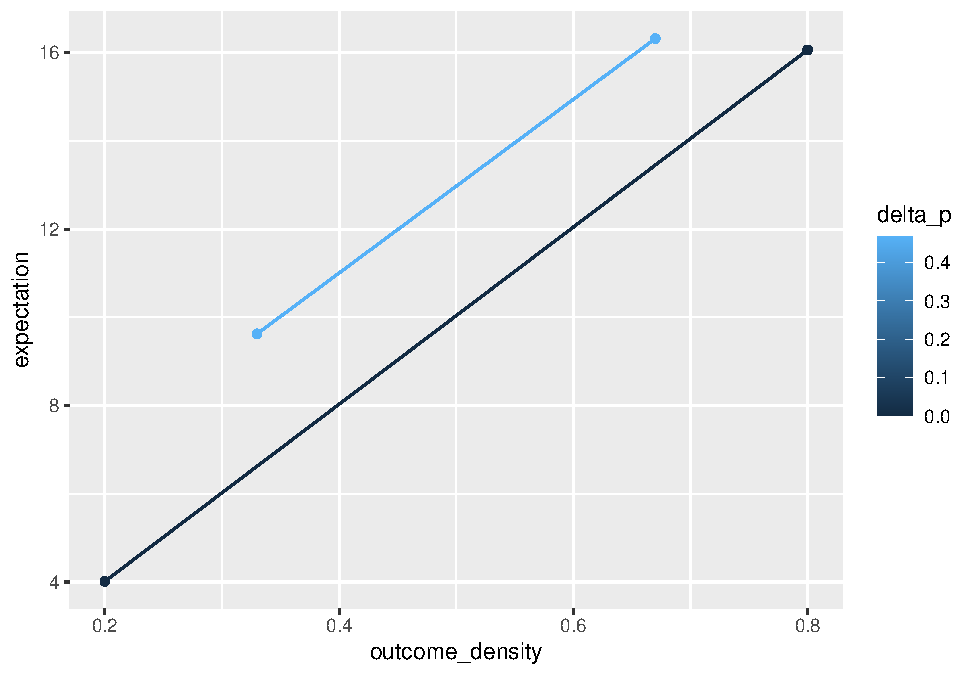
\includegraphics{thesis_files/figure-latex/unnamed-chunk-2-1.pdf}
\caption{\label{fig:unnamed-chunk-2}Write a caption for figure 1}
\end{figure}

\hypertarget{results}{%
\section{Results}\label{results}}

Did our MINERVA model produce a similar \(\triangle\)P effect and outcome density effect to those found in the Crump et al.~(2007) study? While our model did produce the effects, it did so with regard to a higher expectation overall than that of the original study. While the original study contained negative expectations, the model only produced positive expectations, although the overall trend of the results was otherwise almost identical to the original study. For both contingent and noncontingent streams of data, contingency ratings were lower when less outcomes were presented. Just like the human participants in the original study, our computer model also had higher contingency ratings when more outcomes were presented than cues (high outcome density). In contingent conditions (\(\triangle\)P=.467), contingency ratings were much higher overall than noncontingent conditions (\(\triangle\)P=0), which, as intended, paralleled the results of the original study.

Were we able to simulate a theoretical negative contingency condition? A negative contingency condition (\(\triangle\)P=-.467) was not present in the original study. In this condition, the presence of a cue would predict the absence of an outcome. We presented the model with two negative contingency trials, one for both high and low outcome density. Our results show that, in theory, had this been the case in the original study, participants would have least expected the occurrence of an outcome under these conditions. In other words, when compared with the two other conditions, contingency ratings were much lower when the model was presented with a negative contingency. This was true for both the high and low outcome density trials.

\hypertarget{discussion}{%
\section{Discussion}\label{discussion}}

The purposes of this experiment were to create a simulated version of the Crump et al.~(2007) study and additionally to experiment with new theoretical conditions within the simulation. In general, our model was able to replicate several attributes of the in-person study, such as the \(\triangle\)P conditions and the outcome densities associated with them, as well as the overall trend of the data.

Our model contains several key differences when compared with the original study done by Crump et al.~(2007). First, presenting the four possible scenarios to the cue and then asking the model to predict what will happen for each of the six conditions yielded results that were similar to those provided by humans. However, the results provided by humans were lower in expectation than those of the model, although similar in range. Scaling error may account for these differences. Another difference between our model and that of the original study is the number of conditions. We included two additional negative contingency conditions in order to evaluate what would theoretically occur had participants predicted the absence of an outcome despite the presence of a cue.

By studying contingency judgements, we can gain a better understanding of factors that influence learning, memory, and eventually decision making. Our results indicate that there is a relationship between the number of times a result is shown, and one's prediction of whether or not they will get that an outcome will occur based on a certain cue. This general principle may have implications in the world of mental health, such as with disorders such as anxiety and depression. For instance, it could be the case that one develops depressive symptoms due in part to what they expect to happen (outcomes), based on previous experiences (cues). Of course, it would require a substantial amount of further research to properly examine how previous experiences shape mental disorders.

\(x=1\)

\newpage

\hypertarget{references}{%
\section{References}\label{references}}

\begingroup
\setlength{\parindent}{-0.5in}
\setlength{\leftskip}{0.5in}

\hypertarget{refs}{}
\begin{cslreferences}
\leavevmode\hypertarget{ref-crumpContingencyJudgementsFly2007}{}%
Crump, M. J. C., Hannah, S. D., Allan, L. G., \& Hord, L. K. (2007). Contingency judgements on the fly. \emph{The Quarterly Journal of Experimental Psychology}, \emph{60}(6), 753--761. \url{https://doi.org/10/b9jjc4}
\end{cslreferences}

\endgroup


\end{document}
